% Build: tectonic docs/report/report.tex   (figures and tables come from evals/analyze_benchmark.py)
\documentclass[11pt]{article}
\usepackage[margin=1in]{geometry}
\usepackage{fontspec}
\usepackage{xeCJK}
\setCJKmainfont{Noto Serif TC}
\usepackage{microtype}
\usepackage{booktabs}
\usepackage{graphicx}
\usepackage{xcolor}
\usepackage{enumitem}
\usepackage{caption}
\usepackage{xurl}
\usepackage[colorlinks=true,linkcolor=blue!50!black,citecolor=blue!50!black,urlcolor=blue!50!black]{hyperref}
\setlist{nosep,leftmargin=*}
\captionsetup{font=small,labelfont=bf}
\graphicspath{{figures/}}
\newcommand{\code}[1]{\texttt{#1}}
\setlength{\emergencystretch}{2em}

\title{Leave Clear Text Alone:\\Does an Editing Skill Keep Coding Agents from Making\\Open-Source Prose Worse?}
\author{Ting-Hong (Elias) Shieh\\University of Illinois Urbana-Champaign\\\small\url{https://github.com/ting-hong-shieh/polish-open-source-prose}}
\date{October 2026}

\begin{document}
\maketitle

\begin{abstract}
Coding agents asked to polish open-source prose tend to rewrite it. We test whether a
small Agent Skill, polish-open-source-prose v0.2.0, keeps them from making text worse, and
whether it does more than a short instruction. Seven model configurations from Anthropic
and OpenAI ran under five conditions (no instruction, a one-sentence and a three-sentence
instruction, and two versions of the skill) on 49 development cases, 24 held-out cases
written after release, and 21 real pull request descriptions that reviewers at Apache
Airflow, Arrow, DataFusion, and CPython had criticized. Literal checks scored every
output, and two judge models graded the held-out outputs blind. Without an instruction
the models changed 96--98\% of texts that should have been left alone, and the judges
rated 30--44\% of all such outputs harmful. A three-sentence instruction recovered most of
the restraint (81--85\% left unchanged, against 88--92\% with the skill; the difference is
not significant), but it also left unsupported claims in place. On held-out cases the
skill fixed them cleanly about twice as often (0.71--0.76 against 0.34). On the real pull
requests no condition cleanly fixed more than a quarter of the reviewers' critiques.
Without an instruction, 21--38\% of rewrites added facts and 23--27\% damaged needed text,
including other authors' AI disclosure lines; with the skill these fell to 0--1\% and
1--4\%, though it fixed fewer problems than its longer first version. The skill costs 2.5
to 3.3 times as much per run in Claude Code. The cases, scores, judge labels, and scripts
are in the project repository; the real pull request text is not.
\end{abstract}

\section{Introduction}

Contributors now ask coding agents to write and tidy the prose around their code: pull
request descriptions, issue replies, commit messages, documentation, and code comments.
Several large open-source projects have responded with explicit rules. Reviewers in those
projects ask for evidence behind claims, for descriptions that match the change, and for
disclosure of AI use (Section~\ref{sec:reviewers}).

An agent asked to ``polish'' a passage tends to treat the request as an obligation to
change it. That creates two risks that matter more to a reviewer than style does. The
agent may rewrite text that was already clear, which costs review time and can shift
meaning; or it may make the text sound more finished than the work behind it, for
example by turning ``probably'' into ``clearly'' or adding a test result nobody ran.

This report evaluates \emph{polish-open-source-prose}, a small Agent Skill written to
prevent those two failures. Version 0.2.0 has four rules and a final check: leave clear text alone, keep
exact elements exact, do not add facts, and edit only where there is a concrete cost. We
ask:

\begin{enumerate}[leftmargin=3.2em]
  \item[\textbf{RQ1}] How often do current models change text that should be left alone,
    and how much does the skill reduce that?
  \item[\textbf{RQ2}] Does the skill do more than a short instruction that states the same
    intent in one or three sentences?
  \item[\textbf{RQ3}] Does the restraint cost anything on text that does need editing?
  \item[\textbf{RQ4}] Do the results hold on cases written after the skill was frozen and
    on real pull request descriptions that reviewers criticized?
  \item[\textbf{RQ5}] What does the skill cost in time and tokens?
\end{enumerate}

We ran seven model configurations from two vendors under five conditions on three case
sets, scored every output with literal checks, and had two judge models grade the
held-out outputs blind. The cases, scores, judge labels, and scripts are in the
repository; the text of the real pull requests is not, because it belongs to their
authors (Section~\ref{sec:data}).

\section{Background}
\label{sec:reviewers}

\paragraph{Agent Skills.} A skill is a folder with a \code{SKILL.md} file whose
frontmatter description tells the agent when to load it, plus optional reference files
the agent reads on demand. Claude Code and Codex both support the format. Only the
description sits in the context until the skill is used, so a skill's cost is paid on
the tasks that load it.

\paragraph{Project policies on AI-assisted contributions.} The Apache Software
Foundation's generative tooling guidance\footnote{\url{https://www.apache.org/legal/generative-tooling.html}}
allows AI-assisted contributions under conditions and recommends that commit messages
carry a \code{Generated-by:} token. The Rust project adopted an LLM usage
policy\footnote{\url{https://forge.rust-lang.org/policies/llm-usage.html}} that does not
accept pull request descriptions or comments that originate from an LLM, while allowing
some uses, such as private review and translation, with disclosure. Apache Airflow added
review instructions aimed at low-effort AI-generated
contributions,\footnote{\url{https://github.com/apache/airflow/pull/62442}} and the
DataFusion contributor guide has a section on AI-assisted
contributions.\footnote{\url{https://datafusion.apache.org/contributor-guide/index.html\#ai-assisted-contributions}}
A public collection of such policies is maintained on
GitHub.\footnote{\url{https://github.com/melissawm/open-source-ai-contribution-policies}}

None of these policies asks for prose that sounds less machine-written. They ask for
claims that can be checked, descriptions that match the change, and disclosure. That
shaped the skill's scope: version 0.1.0 had grown from a list of phrases typical of model
prose (it drew on stop-slop\footnote{\url{https://github.com/hardikpandya/stop-slop}}),
and version 0.2.0 dropped the phrase lists in favor of rules about fidelity.

\paragraph{What reviewers object to.} To see which problems reviewers raise, we searched
pull request comments in apache/airflow, apache/datafusion, apache/arrow, and
python/cpython from 2025-10-01 to 2026-10-04 for phrases such as ``AI-generated'',
``LLM'', and ``provide evidence'', and saved 459 matching threads with their description
edit history and title changes. A stratified sample of 48 threads was labeled by a Claude
subagent and spot-checked. Figure~\ref{fig:critiques} shows the critique types.
Thirty-three of the 48 threads criticized the text itself, not only the code. The most
common complaints were claims without evidence (24 threads) and undisclosed AI use (19).
Padded or hard-to-read text came up less often (7 and 6 threads). Authors edited the
description or title afterwards in 13 threads. The label ``Other'' (29) covers critiques
of the code, the process, or the contributor's conduct; a thread can carry several labels.

\begin{figure}[t]
  \centering
  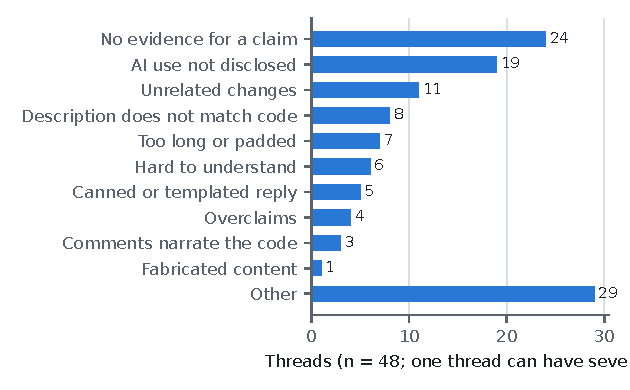
\includegraphics[width=0.62\linewidth]{critiques.pdf}
  \caption{Critique types in 48 labeled review threads from four projects. The sample
    comes from a phrase search, so it shows what reviewers object to, not how often.}
  \label{fig:critiques}
\end{figure}

\section{Related work}

\paragraph{Over-editing.} Studies of grammatical error correction found that ChatGPT tends
to over-correct, producing fluent rewrites where a minimal edit was expected
\cite{fang2023gec}. Our keep cases measure the same tendency in a coding-agent setting,
where the cost is not a lower correction score but a reviewer reading changes nobody asked
for.

\paragraph{Instruction following.} IFEval scores whether a model follows instructions that
can be checked mechanically, such as length or required keywords \cite{zhou2023ifeval}.
Our literal checks follow the same idea for an editing task: strings that must survive,
must go, or must not appear, plus exact equality for text that should not change.

\paragraph{LLM judges.} Using strong models as judges agrees reasonably well with human
preferences but shows position, verbosity, and self-enhancement biases
\cite{zheng2023judge}, and models can recognize and favor their own outputs
\cite{panickssery2024self}. We therefore hide model and condition from the judges, use two
judges from different vendors, report them separately, and measure self-preference
(Section~\ref{sec:judges}).

\paragraph{Detection and provenance.} Detectors of model-written text misclassify writing
by non-native English speakers as machine-generated \cite{liang2023detectors} and can be
defeated by paraphrasing \cite{sadasivan2023detect}. Watermarks such as SynthID-Text are
applied while the model samples tokens \cite{dathathri2024synthid}, so a later editing step
cannot add or certify one. For these reasons the skill does not try to make text sound
human or pass a detector, and v0.2.0 dropped the phrase lists that v0.1.0 had used for
that purpose.

\paragraph{Agent Skills.} Anthropic introduced the skill format with progressive
disclosure: the agent sees each skill's name and description and loads the body when a
task needs it \cite{zhang2025skills}. A study of 238 \code{SKILL.md} files found that over
99\% violate at least one authoring best practice \cite{hong2026skillsmells}. That work
examines how skills are written; this report measures what one skill changes in agent
output, against instructions short enough to put in a prompt.

\section{What we compared}

\paragraph{Conditions.} Every case was run under five conditions. The task prompt was the
same in all of them; only the added instruction differed.

\begin{itemize}
  \item \textbf{No skill}: the task prompt alone.
  \item \textbf{One sentence}: ``If the text is already clear and fits its surface,
    returning it unchanged is a valid answer.''
  \item \textbf{Three sentences}\footnote{The instruction has four sentences; the name
    stuck from an earlier draft.}: ``Polish this text only where there is a concrete
    problem. Leave already-clear text unchanged. Preserve facts, scope, conditions,
    negation, commands, links, quotations, and author voice. Do not invent missing
    facts.''
  \item \textbf{Skill v0.1.0}: the first release, a style guide of 1{,}175 words in
    \code{SKILL.md} plus six reference files (about 3{,}900 words) with English and
    Chinese pattern lists, surface notes, and examples.
  \item \textbf{Skill v0.2.0}: the current release, 943 words in \code{SKILL.md} plus two
    reference files (a Taiwan locale pack and a provenance note, 606 words together).
\end{itemize}

The short instructions were prepended to the task prompt. They were written once, in
English, and not tuned.

\paragraph{Models and harnesses.} Seven configurations: Claude Opus 5.5, Opus 4.6, and
Sonnet 5.5 at high effort in Claude Code; GPT-6.1 Sol at high, GPT-6 Astra at high and
low, and GPT-6 Luna at max reasoning effort in Codex CLI 0.160.0. Claude Code ran with
only the Read and Skill tools, no MCP servers, and no session persistence; skill arms
forced the skill with a slash command naming a project-local copy of the version under
test. Codex ran in a \code{bwrap} sandbox with an empty home directory; skill arms placed
the skill under \code{.agents/skills} with an \code{AGENTS.md} line asking the agent to
use it. Event logs show that every Codex skill run opened \code{SKILL.md}.

Claude configurations ran each case twice per condition and we report the mean of the two
runs; Codex configurations ran once. The two harnesses use different task prompts. Claude
received the task in the case's language and was asked to put the revision inside
\code{<revised>} tags. Codex received the same one-line Chinese task prompt for every case
(inherited from the first experiment), asking for the usable result only, with the
surface and target locale filled in. We therefore compare conditions within a
configuration, not vendors.

\section{Benchmark}
\label{sec:data}

\paragraph{Development set (49 cases).} The skill's own forward cases at commit
\code{2a05713}: 19 \emph{keep} cases whose correct answer is the input unchanged, 26
\emph{rewrite} cases, 2 \emph{audit} cases, and 2 provenance questions (left out of the
scores below). Twenty-one are in English and 28 in Traditional Chinese (Taiwan). The
skill was developed against these cases, and seven expected answers were corrected during
development, so this set measures fit, not generalization.

\paragraph{Held-out set A1 (24 cases).} Written after v0.2.0 was released and frozen at
commit \code{fa993da} before any model ran on it: 8 keep and 8 rewrite cases in English, 4
and 4 in Traditional Chinese. Each case follows the pattern of a real reviewer critique
(linked in the case) but uses new wording and invented project details, and each has a
short rubric. The cases were drafted with Claude Opus 5.5, which is also one of the tested
models.

\paragraph{Held-out set A2 (21 cases).} Real pull request titles and descriptions from
apache/airflow (11), apache/arrow (6), apache/datafusion (2), and python/cpython (2), as
they stood before a reviewer criticized their text, selected from the collected threads.
Each case keeps the reviewer's critique, a description of what a careful editor would do,
and the author's later revision for scoring; the model sees only the original. Critique
kinds: overclaim (6), description does not match the change (4), misleading title (4),
unclear (3), AI-sounding (2), other (2). In 12 of the 21 cases the critique depends on
something outside the text, such as the diff or CI results, so no text-only editor can
fully address it; the best an editor can do there is not make things worse and ask. The
text stays outside Git; \code{evals/heldout/a2\_manifest.json} records the URLs and a
SHA-256 of the case file, committed before any run.

\paragraph{Literal scoring.} Each development and A1 case lists strings that must be
preserved, must be removed, or must not be introduced. Matching is on NFC-normalized,
case-sensitive substrings. A keep case passes only if the output equals the input, apart
from trailing whitespace.

\paragraph{Judged scoring.} Two judges, Claude Opus 5.5 and GPT-6.1 Sol at high effort and
without the skill, graded outputs blind: all outputs for one case were shuffled under
random labels and graded in groups of up to 20. For A1 and A2 edit cases the judge saw the
original, the rubric (A1) or the reviewer's critique and ideal behavior (A2), and each
output's revised text. It decided whether the output addressed the problem (0, 0.5, or 1),
invented a fact, or damaged something needed. Claude Code outputs usually carried a note
to the author outside the \code{<revised>} tags, such as a question about where a number
came from. The judge saw that note too: a question in it counted toward addressing a
problem the text alone cannot fix, but only the revised text counted for invented or
damaged facts. The Codex prompt asked for the usable result only, so Codex outputs had no
such channel. For keep cases in the development set and A1, every output that changed
the text was judged for whether the change was harmful: whether it altered meaning, a
fact, a condition, scope, an obligation, a quotation, an identifier, or the author's
voice, or added information. Both judges are also tested models, so we report them
separately and check for self-preference (Section~\ref{sec:judges}).

\section{Results}

Tables~\ref{tab:main} and~\ref{tab:a1} give literal pass rates for every configuration and
condition. Figure~\ref{fig:tradeoff} pools the seven configurations, giving each the same
weight, with 95\% intervals from resampling cases.

\begin{table*}[t]\centering\small
\caption{Development set: percentage of cases passing, by model and condition (mean over runs; 19 keep and 28 edit cases; the 2 provenance cases are left out).}\label{tab:main}
\begin{tabular}{lrrrrrrrrrr}
\toprule
 & \multicolumn{2}{c}{No skill} & \multicolumn{2}{c}{One sentence} & \multicolumn{2}{c}{Three sentences} & \multicolumn{2}{c}{Skill v0.1.0} & \multicolumn{2}{c}{Skill v0.2.0} \\
\cmidrule(lr){2-3}\cmidrule(lr){4-5}\cmidrule(lr){6-7}\cmidrule(lr){8-9}\cmidrule(lr){10-11}
 & keep & edit & keep & edit & keep & edit & keep & edit & keep & edit \\
\midrule
Opus 5.5 & 8 & 73 & 68 & 79 & 82 & 64 & 71 & 75 & 100 & 89 \\
Opus 4.6 & 8 & 68 & 76 & 68 & 82 & 43 & 50 & 88 & 95 & 84 \\
Sonnet 5.5 & 16 & 68 & 79 & 71 & 92 & 61 & 92 & 82 & 100 & 89 \\
GPT-6.1 Sol & 0 & 64 & 42 & 54 & 79 & 43 & 32 & 82 & 95 & 89 \\
GPT-6 Astra (high) & 0 & 57 & 42 & 64 & 90 & 50 & 26 & 75 & 100 & 93 \\
GPT-6 Astra (low) & 0 & 61 & 16 & 57 & 79 & 43 & 10 & 71 & 100 & 93 \\
GPT-6 Luna (max) & 0 & 36 & 37 & 39 & 63 & 39 & 5 & 57 & 53 & 68 \\
\bottomrule
\end{tabular}
\end{table*}

\begin{table*}[t]\centering\small
\caption{Held-out set A1: percentage of cases passing literal checks (12 keep, 12 edit).}\label{tab:a1}
\begin{tabular}{lrrrrrrrrrr}
\toprule
 & \multicolumn{2}{c}{No skill} & \multicolumn{2}{c}{One sentence} & \multicolumn{2}{c}{Three sentences} & \multicolumn{2}{c}{Skill v0.1.0} & \multicolumn{2}{c}{Skill v0.2.0} \\
\cmidrule(lr){2-3}\cmidrule(lr){4-5}\cmidrule(lr){6-7}\cmidrule(lr){8-9}\cmidrule(lr){10-11}
 & keep & edit & keep & edit & keep & edit & keep & edit & keep & edit \\
\midrule
Opus 5.5 & 0 & 33 & 71 & 42 & 79 & 62 & 79 & 75 & 96 & 83 \\
Opus 4.6 & 12 & 38 & 58 & 58 & 79 & 50 & 54 & 54 & 92 & 71 \\
Sonnet 5.5 & 4 & 46 & 92 & 58 & 92 & 58 & 88 & 75 & 92 & 83 \\
GPT-6.1 Sol & 0 & 42 & 25 & 25 & 83 & 25 & 0 & 50 & 92 & 75 \\
GPT-6 Astra (high) & 0 & 33 & 33 & 42 & 92 & 42 & 8 & 42 & 92 & 92 \\
GPT-6 Astra (low) & 0 & 50 & 8 & 33 & 100 & 25 & 0 & 42 & 92 & 92 \\
GPT-6 Luna (max) & 0 & 33 & 33 & 33 & 67 & 17 & 0 & 25 & 58 & 58 \\
\bottomrule
\end{tabular}
\end{table*}


\begin{figure}[t]
  \centering
  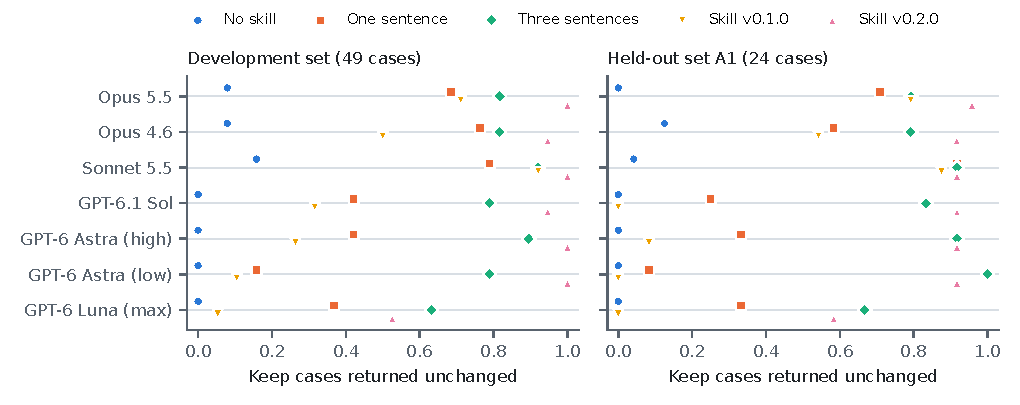
\includegraphics[width=\linewidth]{keep.pdf}
  \caption{Share of keep cases returned unchanged, by configuration and condition.}
  \label{fig:keep}
\end{figure}

\subsection{RQ1: Models rewrite clear text unless told not to}

With no added instruction, every configuration changed almost every keep case: 0--16\%
were returned unchanged on the development set and 0--12\% on A1 (Figure~\ref{fig:keep}).
Many of those changes were not harmless rewording. The judges rated 39--44\% of all
no-skill outputs on development keep cases, and 30--38\% on A1, as changing meaning, a
fact, a condition, an obligation, an identifier, or the author's voice
(Figure~\ref{fig:harm}). Changes that both judges rated harmful include translating an
English license notice into Chinese, adding a confirmation step to an ordered procedure,
adding a disclosure condition to a security policy, replacing a colloquial phrase that
was the author's voice, and turning ``tested'' into ``verified''.

With v0.2.0, six of the seven configurations returned 92--100\% of keep cases unchanged on
both sets. GPT-6 Luna at max effort was the exception, at 53\% and 58\%: it still
translated license text, replaced the UI label, and reworded commit references.

\begin{figure}[t]
  \centering
  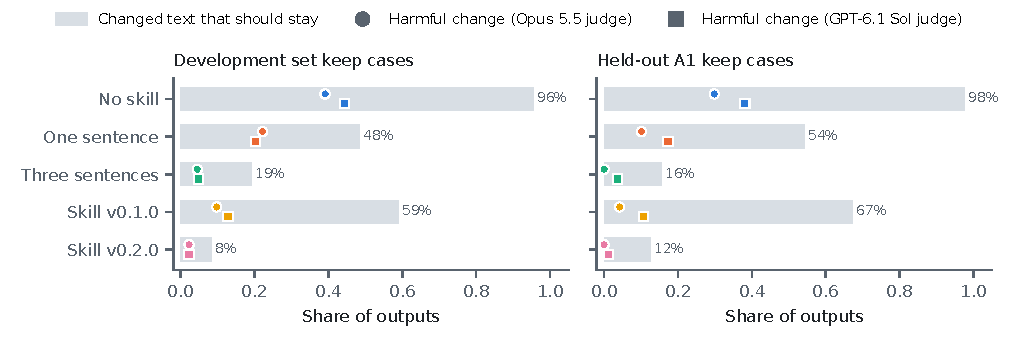
\includegraphics[width=\linewidth]{harm.pdf}
  \caption{Keep cases: the bar is the share of outputs that changed the text; the markers
    are the share of all outputs whose change a judge rated harmful.}
  \label{fig:harm}
\end{figure}

\subsection{RQ2: A three-sentence instruction recovers most of the restraint}

Pooled over configurations, the three-sentence instruction left 81\% of development keep
cases unchanged (95\% interval 69--91\%) and 85\% of A1 keep cases (69--96\%), against 92\%
(87--95\%) and 88\% (72--98\%) for v0.2.0. The difference is not significant: v0.2.0 did
better on 8 development cases and worse on 2 ($p=0.11$), and better on 2 A1 cases and worse
on 3 ($p=1$; Table~\ref{tab:signs}). The judged harm rates are low for both: 4--5\% for the
three-sentence instruction and 2\% for v0.2.0 on the development set, and at most 4\% and
1\% on A1.

The one-sentence instruction was much weaker (52\% and 46\% unchanged). Version 0.1.0, the
longer style guide, was weaker still on this measure (41\% and 33\%): for the four GPT
configurations it left fewer keep cases unchanged than the one-sentence instruction did.
A style guide full of patterns to fix plausibly gives the model more reasons to edit.

\subsection{RQ3: The short instruction gives up the edits that matter}

The three-sentence instruction pays for its restraint on text that does need work. On
edit cases it passed 49\% of literal checks on the development set and 40\% on A1, no better
than no instruction (61\% and 39\%), while v0.2.0 passed 86\% and 79\%
(Figure~\ref{fig:tradeoff}). Against the three-sentence instruction, v0.2.0 did better on
20 development edit cases and worse on 1 ($p<0.001$), and better on 9 A1 edit cases and
worse on 1 ($p=0.02$).

The judges explain why (Table~\ref{tab:judged}). Under the three-sentence instruction the
models returned 56\% of A1 edit cases unchanged, leaving claims such as ``3x faster'' with
no benchmark, or ``fully tested and safe to merge'' after one test file, in place. In
some of these the model's own note named the problem and kept the text anyway, because the
instruction said to leave clear text unchanged (Appendix~\ref{app:examples}). Its mean
score for addressing the problem was 0.34 from both judges, against 0.76--0.77 for v0.2.0.
Without any instruction the models addressed more problems (0.60--0.61), but 11--19\% of
their outputs added a fact the author had not given, against 1\% for v0.2.0. Counting a
fix only when the revision neither added a fact nor damaged needed text (a \emph{clean
fix}), v0.2.0 scored 0.71--0.76, the three-sentence instruction 0.34, and no instruction
0.45--0.49; v0.2.0 did better than both on most cases (12:0 and 10:1;
Table~\ref{tab:signs}). Version 0.1.0 came close (0.67--0.71; 9:3, $p=0.15$). The skill
differs from the short instruction in naming what counts as a problem: unsupported
certainty, quality claims without evidence, and test results stretched beyond their
scope.

\begin{figure}[t]
  \centering
  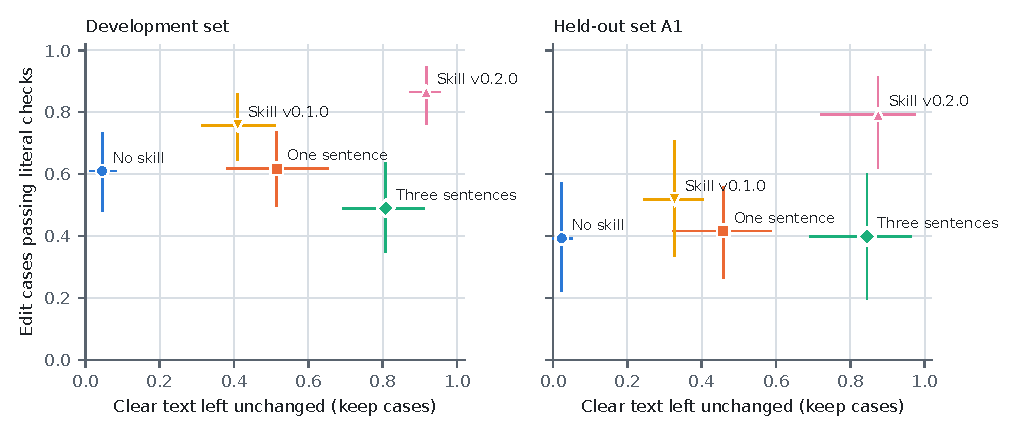
\includegraphics[width=\linewidth]{tradeoff.pdf}
  \caption{Keep cases left unchanged against edit cases passing literal checks, pooled over
    seven configurations. Bars are 95\% intervals from resampling cases.}
  \label{fig:tradeoff}
\end{figure}

\begin{table}[t]\centering\small
\caption{Paired sign tests of v0.2.0 against each other condition: cases where v0.2.0 scored better:worse (two-sided $p$). Each case's score is averaged over the seven configurations, their runs, and, for judged scores, both judges; ties are dropped.}\label{tab:signs}
\begin{tabular}{lrrrr}
\toprule
 & No skill & One sentence & Three sentences & Skill v0.1.0 \\
\midrule
Development, keep (literal) & 19:0 (<.001) & 17:0 (<.001) & 8:2 (.109) & 19:0 (<.001) \\
Development, edit (literal) & 17:4 (.007) & 19:2 (<.001) & 20:1 (<.001) & 13:4 (.049) \\
A1, keep (literal) & 12:0 (<.001) & 11:0 (<.001) & 2:3 (1.000) & 12:0 (<.001) \\
A1, edit (literal) & 11:1 (.006) & 11:0 (<.001) & 9:1 (.021) & 9:0 (.004) \\
A1, edit (judged clean fix) & 10:1 (.012) & 10:1 (.012) & 12:0 (<.001) & 9:3 (.146) \\
A2, edit (judged clean fix) & 10:7 (.629) & 9:5 (.424) & 12:1 (.003) & 4:9 (.267) \\
\bottomrule
\end{tabular}
\end{table}


\begin{figure}[t]
  \centering
  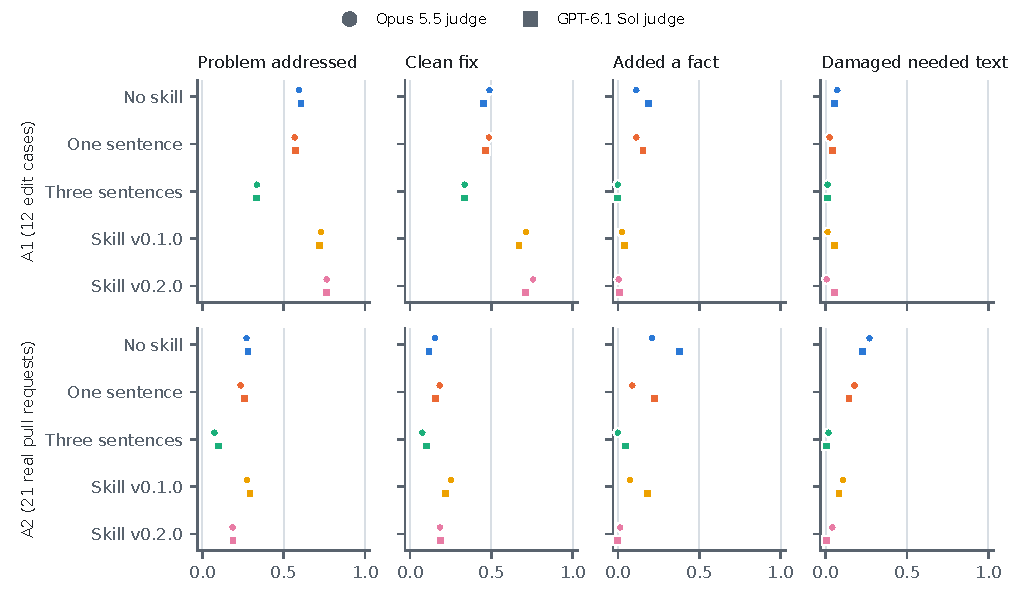
\includegraphics[width=\linewidth]{judged.pdf}
  \caption{Judged edit cases in A1 and A2. A clean fix counts the addressed score only
    when the revision neither added a fact nor damaged needed text.}
  \label{fig:judged}
\end{figure}

\begin{table*}[t]\centering\small
\caption{Judged edit cases. In each pair the first number is from the Opus 5.5 judge and the second from the GPT-6.1 Sol judge. \emph{Addressed} and \emph{clean fix} are mean scores from 0 to 1; a clean fix counts the addressed score only when the revision neither added a fact nor damaged needed text. \emph{Added a fact}, \emph{damaged}, and \emph{unchanged} are percentages of outputs. Models weigh equally; Claude runs are averaged first.}\label{tab:judged}
\begin{tabular}{lrrrrrrrrr}
\toprule
 & \multicolumn{2}{c}{Addressed} & \multicolumn{2}{c}{Clean fix} & \multicolumn{2}{c}{Added a fact} & \multicolumn{2}{c}{Damaged} & Unchanged \\
\cmidrule(lr){2-3}\cmidrule(lr){4-5}\cmidrule(lr){6-7}\cmidrule(lr){8-9}
\midrule
\multicolumn{10}{l}{\emph{A1 (12 cases)}} \\
\quad No skill & 0.59 & 0.61 & 0.49 & 0.45 & 11 & 19 & 7 & 5 & 0 \\
\quad One sentence & 0.57 & 0.57 & 0.48 & 0.46 & 11 & 16 & 2 & 4 & 15 \\
\quad Three sentences & 0.34 & 0.34 & 0.34 & 0.34 & 0 & 0 & 1 & 1 & 56 \\
\quad Skill v0.1.0 & 0.73 & 0.72 & 0.71 & 0.67 & 2 & 4 & 1 & 5 & 9 \\
\quad Skill v0.2.0 & 0.77 & 0.76 & 0.76 & 0.71 & 1 & 1 & 1 & 5 & 12 \\
\multicolumn{10}{l}{\emph{A2 (21 real pull requests)}} \\
\quad No skill & 0.27 & 0.28 & 0.15 & 0.12 & 21 & 38 & 27 & 23 & 0 \\
\quad One sentence & 0.24 & 0.26 & 0.18 & 0.15 & 9 & 22 & 18 & 14 & 7 \\
\quad Three sentences & 0.07 & 0.10 & 0.07 & 0.10 & 0 & 5 & 2 & 1 & 13 \\
\quad Skill v0.1.0 & 0.28 & 0.29 & 0.25 & 0.22 & 8 & 18 & 10 & 8 & 4 \\
\quad Skill v0.2.0 & 0.19 & 0.19 & 0.18 & 0.19 & 1 & 0 & 4 & 1 & 24 \\
\bottomrule
\end{tabular}
\end{table*}


\subsection{RQ4: On real pull requests, the skill avoids harm but fixes little}

Real descriptions were much harder (Figure~\ref{fig:judged}). No condition scored above
0.3 for addressing the reviewer's critique. Twelve of the 21 critiques depended on
something outside the text, such as the diff or a CI run; on the 9 that could be judged
from the text alone the best score was still under 0.39.

Without an instruction the models addressed critiques about as often as with v0.1.0
(0.27--0.28 against 0.28--0.29), but 21--38\% of their outputs added a fact and 23--27\% damaged needed
text. Changes that both judges flagged include narrowing an access rule from ``other''
DAGs to ``unauthorized'' ones, deleting an SPDX license header, and editing the author's
AI disclosure. Seven A2 descriptions carry Airflow's \code{Generated-by:} disclosure line.
Across their 70 outputs per condition, that line was altered or deleted 10 times without
an instruction, 9 times with one sentence, once each with three sentences and v0.1.0, and
never with v0.2.0. GPT models added ChatGPT or Codex to another author's disclosure in 8
outputs, and GPT-6 Luna deleted the line in 5.

With v0.2.0, outputs almost never added a fact (0--1\%) or damaged needed text (1--4\%),
but the skill addressed fewer critiques (0.19) and left 24\% of descriptions unchanged.
On clean fixes it scored 0.18--0.19: above no instruction (0.12--0.15) and the
three-sentence instruction (0.07--0.10), and below v0.1.0 (0.22--0.25). Only the
difference from the three-sentence instruction is significant (12:1, $p=0.003$; against
no instruction 10:7, $p=0.63$; against v0.1.0 4:9, $p=0.27$). By critique type, v0.2.0
fell furthest behind on misleading titles (0.13 against 0.38 without an instruction, 4
cases) and on text reviewers called AI-sounding (0.07 against 0.21, 2 cases): style
problems that v0.2.0 stopped targeting. With so few cases, read this as a direction to
check, not a result.

\subsection{Judge agreement}
\label{sec:judges}

The two judges agreed closely on whether an edit addressed the problem (exact agreement
91\%, weighted $\kappa=0.93$, 1{,}650 outputs) and on whether a change to a keep case was
harmful (88.5\%, $\kappa=0.73$, 667 outputs). They agreed less on added facts ($\kappa=0.59$;
the Sol judge flagged 14\% of outputs and the Opus judge 7\%) and on damage
($\kappa=0.46$), so Table~\ref{tab:judged} reports both. Neither judge favored its own
model by much. The Opus 5.5 judge scored Opus 5.5 outputs 0.018 higher than the Sol judge
did, against $-0.011$ for other models' outputs; the Sol judge scored Sol outputs 0.021
higher than the Opus judge did, against 0.003 for the rest. These gaps are small next to
the differences between conditions. A first pass on A1 that hid the editor's note from
the judges gave the same order: 0.73 for v0.2.0, 0.30--0.32 for the three-sentence
instruction, and 0.58--0.59 without an instruction.

\subsection{RQ5: Cost}

Loading the skill costs time and tokens on every task that uses it
(Table~\ref{tab:cost}). In Claude Code, a v0.2.0 run cost 2.5 to 3.3 times as much as a
run without it (Opus 5.5: \$0.123 against \$0.044) and took 3--9 seconds longer. In Codex,
input tokens rose from about 11--12k to 27--28k and run time from 11--16 to 18--38 seconds.
Version 0.1.0 used more tokens than v0.2.0 in every configuration. The short
instructions cost nothing measurable.

\begin{table}[t]\centering\small
\caption{Mean seconds and cost per run on the held-out sets. Claude cost is the API-equivalent estimate that Claude Code reports, not a bill; for Codex the table gives input tokens.}\label{tab:cost}
\begin{tabular}{lrrrrrr}
\toprule
 & \multicolumn{2}{c}{No skill} & \multicolumn{2}{c}{Three sentences} & \multicolumn{2}{c}{Skill v0.2.0} \\
\cmidrule(lr){2-3}\cmidrule(lr){4-5}\cmidrule(lr){6-7}
 & s & cost & s & cost & s & cost \\
\midrule
Opus 5.5 & 14 & \$0.044 & 12 & \$0.039 & 17 & \$0.123 \\
Opus 4.6 & 13 & \$0.038 & 18 & \$0.044 & 22 & \$0.093 \\
Sonnet 5.5 & 9 & \$0.018 & 8 & \$0.018 & 12 & \$0.059 \\
GPT-6.1 Sol & 15 & 12.0k & 18 & 12.0k & 23 & 28.4k \\
GPT-6 Astra (high) & 12 & 11.9k & 14 & 11.9k & 19 & 28.3k \\
GPT-6 Astra (low) & 11 & 11.9k & 13 & 11.9k & 18 & 28.3k \\
GPT-6 Luna (max) & 16 & 11.3k & 22 & 11.3k & 38 & 27.0k \\
\bottomrule
\end{tabular}
\end{table}


\section{Discussion}

\paragraph{What the skill adds.} For leaving clear text alone, not much beyond a short
instruction. Three sentences in a prompt got most configurations to 79--100\% on keep
cases at no extra cost. The skill's measurable contribution is on text that does need an
edit. A short instruction to edit ``only where there is a concrete problem'' does not say
what a problem is, and the models read it as permission to leave unsupported claims in
place. The skill names the problems that reviewers in Section~\ref{sec:reviewers} raise
most, and on held-out text it fixed them cleanly about twice as often as the
three-sentence instruction did.

\paragraph{When to use which.}
\begin{itemize}
  \item If an agent mostly touches text that is already fine, such as tidying or
    translating documentation, put the three-sentence instruction in \code{AGENTS.md} or
    \code{CLAUDE.md}.
  \item If it drafts or revises pull request descriptions, release notes, or review
    replies, where overclaims are likely, the skill catches more of them at 2.5 to 3.3
    times the cost per run.
  \item With either, read the output. GPT-6 Luna at max effort ignored the skill's first
    rule on about half of the keep cases.
\end{itemize}

\paragraph{What the skill does not do.} It does not make text sound human and cannot
supply evidence the author did not give. In A2, most of what reviewers objected to needed facts only
the author had: the diff, the CI run, the benchmark. No condition cleanly fixed more than a
quarter of those critiques. What v0.2.0 did reliably on real descriptions was not make them
worse, including leaving other people's disclosure lines alone. It also fixed fewer
problems than v0.1.0, mostly misleading titles and text reviewers called AI-sounding.
That is the cost of its narrower scope and the first place to look in a next version.

\paragraph{A lesson from v0.1.0.} The longer first version, built around lists of patterns
to fix, made models edit more, not better. For the GPT configurations it left fewer clear
texts alone than the one-sentence instruction did, and it used more tokens than v0.2.0
everywhere. Rules about when not to edit did more than lists of what to fix.

\section{Threats to validity}
\label{sec:threats}

\begin{itemize}
  \item \textbf{Who wrote the cases.} The development set was written by the maintainer
    with an AI assistant, and the skill was tuned on it. A1 was drafted by Claude Opus 5.5
    after release and shares its authors' idea of a good edit; the literal checks for A1
    edit cases encode that idea. A2 and the judges are the checks against this, and A2 is
    small.
  \item \textbf{Scope of A2.} Twenty-one English pull request descriptions from four
    projects, found by phrase search. They do not cover documentation, comments, or other
    languages.
  \item \textbf{Literal scoring} misses paraphrases that keep the meaning and counts a
    harmless fix to clear text as a failure. The judged harm rate on keep cases separates
    those.
  \item \textbf{Judges.} Both judges are tested models and share training-era habits with
    the editors they grade. Labels were blind to model and condition.
  \item \textbf{Sample size.} Claude configurations ran twice and Codex configurations
    once, so per-model results are noisy, and A1 and A2 have 24 and 21 cases. The pooled tests use cases as the unit and treat
    the seven configurations as fixed.
  \item \textbf{Harness asymmetry.} Task prompts, output format, and skill activation
    differ between Claude Code and Codex. Claude outputs could carry a note to the author
    and Codex outputs could not, which favors Claude where the right move is to ask.
    Within-configuration comparisons are unaffected; cross-vendor comparisons are not
    meaningful.
  \item \textbf{Baselines.} The short instructions are in English and were not tuned. A
    better short instruction may close part of the gap reported here.
  \item \textbf{Earlier runs.} An earlier report on GPT-6 Astra used a sandbox in which
    the agent could not run shell commands, so it never read the skill's reference files.
    Those runs are not used here; all Codex skill runs in this report opened
    \code{SKILL.md}.
\end{itemize}

\section{Conclusion}

Current models rewrite clear text by default, and much of that rewriting changes meaning.
A three-sentence instruction prevents most of it at no cost. The polish-open-source-prose
skill adds two things the short instruction does not: it fixes unsupported claims instead
of leaving them in place, and on real pull request descriptions it almost never adds a
fact or alters a disclosure. It does not fix most of what reviewers object to, because
most of that needs facts only the author has.

For a contributor the practical advice is short. Tell the agent to leave clear text alone
and not to add facts. Use the skill when the agent writes claims about your change. Then
check what it wrote against what you did.

\section*{Use of AI tools}

The experiments were carried out with Claude Code running Claude Opus 5.5, under the
author's direction. It wrote the scoring, judging, and analysis scripts, drafted the A1
cases, labeled the sample of review threads, ran the models, and drafted this report. The
author chose the research questions, conditions, models, and data sources, approved each
step before it ran, and takes responsibility for the content. Claude Opus 5.5 is also one
of the tested models and one of the two judges; Sections~\ref{sec:judges}
and~\ref{sec:threats} discuss what that may bias.

\begin{thebibliography}{99}\small
\bibitem{dathathri2024synthid} S.~Dathathri, A.~See, S.~Ghaisas, P.-S.~Huang, et al.
  Scalable watermarking for identifying large language model outputs.
  \emph{Nature}, 634:818--823, 2024.
\bibitem{fang2023gec} T.~Fang, S.~Yang, K.~Lan, D.~F.~Wong, J.~Hu, L.~S.~Chao, and Y.~Zhang.
  Is ChatGPT a highly fluent grammatical error correction system? A comprehensive
  evaluation. arXiv:2304.01746, 2023.
\bibitem{hong2026skillsmells} D.~B.~Hong, A.~Imani, and I.~Ahmed.
  From anatomy to smells: An empirical study of SKILL.md in Agent Skills.
  arXiv:2607.01456, 2026.
\bibitem{liang2023detectors} W.~Liang, M.~Yuksekgonul, Y.~Mao, E.~Wu, and J.~Zou.
  GPT detectors are biased against non-native English writers.
  \emph{Patterns}, 2023. arXiv:2304.02819.
\bibitem{panickssery2024self} A.~Panickssery, S.~R.~Bowman, and S.~Feng.
  LLM evaluators recognize and favor their own generations. arXiv:2404.13076, 2024.
\bibitem{sadasivan2023detect} V.~S.~Sadasivan, A.~Kumar, S.~Balasubramanian, W.~Wang, and
  S.~Feizi. Can AI-generated text be reliably detected?
  \emph{Transactions on Machine Learning Research}, 2025. arXiv:2303.11156.
\bibitem{zhang2025skills} B.~Zhang, K.~Lazuka, and M.~Murag.
  Equipping agents for the real world with Agent Skills. Anthropic Engineering, October
  2025. \url{https://www.anthropic.com/engineering/equipping-agents-for-the-real-world-with-agent-skills}
\bibitem{zheng2023judge} L.~Zheng, W.-L.~Chiang, Y.~Sheng, S.~Zhuang, Z.~Wu, et al.
  Judging LLM-as-a-judge with MT-Bench and Chatbot Arena.
  In \emph{NeurIPS Datasets and Benchmarks Track}, 2023. arXiv:2306.05685.
\bibitem{zhou2023ifeval} J.~Zhou, T.~Lu, S.~Mishra, S.~Brahma, S.~Basu, Y.~Luan, D.~Zhou,
  and L.~Hou. Instruction-following evaluation for large language models.
  arXiv:2311.07911, 2023.
\end{thebibliography}

\appendix
\section{Reproducing}

Raw runs, event logs, and the A2 cases live under \code{\$POLISH\_EVAL\_DATA} (see
\code{evals/README.md}). From the repository root:

\begin{verbatim}
POLISH_EVAL_DATA=/mnt/d/Data python3 evals/score_benchmark.py
POLISH_EVAL_DATA=/mnt/d/Data python3 evals/judge_outputs.py --judge both
POLISH_EVAL_DATA=/mnt/d/Data .venv/bin/python evals/analyze_benchmark.py
tectonic docs/report/report.tex
\end{verbatim}

The judge script calls the \code{claude} and \code{codex} command-line tools; set
\code{CLAUDE\_BIN}, \code{CODEX\_BIN}, and \code{CODEX\_AUTH} if they are not on the path.
\code{evals/results/benchmark.json} holds every scored output for the development set and
A1, and \code{evals/results/judgments.json} every judge label for them. A2 outputs and
labels stay with the A2 cases. \code{evals/results/analysis.json} holds the aggregates in
this report, including A2.

\section{Examples from held-out set A1}
\label{app:examples}

Outputs are verbatim from the first run. Both cases are English pull request text. Claude
Code outputs also carried a note to the author, summarized here.

\paragraph{An unsupported speedup.} Input: ``This avoids copying each batch twice in
\code{SortExec}, which makes queries 3x faster.'' The rubric: the speedup has no
benchmark, data size, or command; keep the mechanism, and drop the number or ask where it
came from.

\begin{itemize}
  \item Opus 5.5, no skill: ``This change stops \code{SortExec} from copying each batch
    twice. On [benchmark or query set], queries ran about 3x faster.'' The note asks the
    author to fill in the placeholder, which sits inside the text meant to be pasted.
  \item Opus 5.5, three sentences: unchanged. The note calls the sentence ``already clear
    and correct'' and suggests naming the benchmark.
  \item Opus 5.5, v0.2.0: ``This avoids copying each batch twice in \code{SortExec}.'' The
    note explains the removal and asks what was measured, the numbers, and which queries
    speed up.
  \item GPT-6.1 Sol, v0.2.0: unchanged, with no note. The skill does not always work.
\end{itemize}

\paragraph{A test result stretched into a conclusion.} Input: ``I ran
\code{pytest tests/test\_xcom.py} and everything passes, so the change is fully tested and
safe to merge.'' The rubric: one test file passing does not make the change fully tested
or safe to merge; keep the command and its result and drop the conclusion.

\begin{itemize}
  \item Opus 5.5, no skill: ``I ran \code{pytest tests/test\_xcom.py} locally, and all tests
    pass.'' Both judges flagged ``locally'' as a fact the author did not give.
  \item Opus 5.5, three sentences: unchanged. The note says that one test file passing
    does not prove the change is ``fully tested and safe to merge'', but leaves the
    sentence as it was because it ``is clear and grammatical''. The model saw the problem
    and kept it, as the instruction to leave clear text unchanged allowed.
  \item Opus 5.5, v0.2.0: ``I ran \code{pytest tests/test\_xcom.py} and all tests in that
    file pass.'' The note asks which commit the tests ran on, whether other tests ran, and
    whether CI passed. Both judges marked this as addressed, but it fails the literal
    check because ``all tests'' is on the case's must-not-introduce list: literal scoring
    counted a good edit as a failure.
\end{itemize}

\end{document}
